\section{HTTP Method Request}
\subsection{Pengertian HTTP Method Request}
Protokol HTTP adalah protokol permintaan atau respon. Klien mengirimkan permintaan keserver dalam bentuk metode permintaan, URL, dan versi protokol, diikuti oleh pesan seperti MIME yang berisi perubahan permintaa, informasi klien, dan kemungkinan onten tubuh melalui koneksi dengan server\cite{wyler2005aggressive}. Protokol ini sangat ringan serta generik dan tidak berstatus sehingga dapat dipergunakan oleh tipe dokumen apa saja. Method adalah sekumpulan kode yang diberi namma, untuk merujuk kesekumpulan kode yang ada kemuadian digunakan sebuah nama yang disebut dengan nama method. Method sendiri mempunyai parameter sebagai input (masukan) dan nilai kembalian sebagai output (keluaran). Request adalah permiintaan dimana fungsi ini digunakan sebagai istilah ataupun kinerja dalam pengembalian nilai dari masukan yang dieksekusi.

Berdasarkan beberapa penjelasann diatas, maka untuk pengertian dari HTTP Method Request sendiri merupakan seperangkat metode permintan untuk menunjukkan tindakan yang diinginkan yang akan dilakukan untuk sumber daya tertentu. Meskipun mereka juga bisa menjadi kata benda, metode permintaan ini kadang-kadang disebut sebagai verba HTTP. Masing-masing menerapkan semantik yang berbeda, namun beberapa fitur umum digunakan bersama oleh mereka adalah misalnya Metode pertmintaan dapat berupa safe, idempotent, atau cacheable.

\subsection{Jenis-jenis HTTP Method Request}
\begin{enumerate}
  \item GET : akan dijelaskan pada point berikutnya.
  \item HEAD : Metode HEAD meminta tanggapan yang identik dengan permintaan GET, namun tanpa respon body.
  \item POST : Metode POST digunakan untuk mengirimkan entitas ke sumber daya yang ditentukan, sering menyebabkan perubahan pada keadaan atau efek samping pada server.
  \item PUT : Metode PUT menggantikan semua representasi terkini dari sumber target dengan muatan permintaan.
  \item DELETE : Metode DELETE akan menghapus sumber daya yang ditentukan
  \item CONNECT : Metode CONNECT menetapkan terowongan keserver yang diidentifikasi oleh sumber target.
  \item OPTIONS : Metode OPTIONS digunakan untuk menggambarkan opsi komunikasi untuk sumber target.
  \item TRACE : metode TRACE ini yaitu untuk melakukan tes pesan loop-back disepanjang jalan menuju sumber daya target.
  \item PATCH : Metode PATCH digunakan untuk menerapkan modifikasi sebagian pada sumber daya.
\end{enumerate}

\subsection{Penjelasan Lengkap HTTP Get Method}
Metode GET digunakan untuk meminta representasi suber daya yang ditentukan. permintaan menggunakan Get seharusnya hanya mengambil data. GET adalah salah satu metode HTTP yang paling umum digunakan baik dalam pengimplementasian biasa ataupun sudah dalam bentuk pengujian. Hal yang harus diperhatikan dalam Method Get yaitu :
\begin{itemize}
  \item Permintaan GET dapat di-cache.
  \item Permintaan GET tetap ada dalam riwayat browser.
  \item Permintaan GET dapat ditandai.
  \item Permintaan GET tidak boleh digunakan saat berurusan dengan data sensitif.
  \item Permintaan GET memiliki batasan panjang.
  \item Permintaan GET hanya digunakan untuk meminta data (tidak dimodifikasi).
  \item Permintaan GET dibatasi oleh panjang string sebanyak 2047 karakter.
  \item Permintaan GET memungkinkan pengunjung langsung memasukkan nilai variable pada form proses.
\end{itemize}

\subsection{Pembacaan HTTP Get Method}
Data dikirimkan dalam HTTP Request dalam dua cara, tergantung dari method yang dikirimkan, yaitu :
\begin{enumerate}
  \item Melalui URL, dengan parameter yang diberikan. Digunakan oleh GET.
  \item Melalui entity body dalam HTTP Request. Digunakan untuk POST dan PUT.
\end{enumerate}

Pada prakteknya terdapat satu cara lagi untuk mengirimkan data, yaitu melalui cookie, tetapi penggunaan cookie tidak akan terlalu efektif karena cookie dirancang untuk menyimpan data status pengguna.

\subsection{Pembacaan Data pada URL}
Pembacaan data yang dikirimkan melalui URL biasanya dilakukan untuk request dengan method GET. Untuk melihat bagaimana GET mengirimkan data, kita terlebih dahulu harus mengerti tentang sintaks penulisan URL. Secara umum, sebuah URL memiliki sintaks seperti berikut :
\lstinputlisting[caption=Contoh kode untuk schema,label={lst:schema}]{src/10/schema.py}
Apa makna dari setiap bagian dari URL yang dijelaskan pada \ref{lst:schema}? Pada tabel \ref{table:schema}, anda dapat melihat makna dan maksud dari contoh URL yang telah diberikan.
\begin{table}[]
\caption{Penjelasan Schema}
\centering
\begin{tabular}{|l|l|l|}
\hline
Nama & Deskripsi & Harus ada ?\\ \hline
schema & Protokol yang digunakan & Ya\\ \hline
user & Nama pengguna & Tidak\\ \hline
password & Password untuk nama pengguna & Tidak\\ \hline
hots & Hostname atau IP & Ya\\ \hline
port & \begin{tabular}[c]{@{}l@{}}Port yang akan diakses. Beberapa atau sebagian\\ protokol memiliki port standar yaitu seperti HTTP = 80\end{tabular} & Tergantung Protokol\\ \hline
paht & Lokasi data pada server & Tergantung Protokol\\ \hline
query & \begin{tabular}[c]{@{}l@{}}Digunakan untuk mengirimkan \\ parameter kepada aplikasi.\end{tabular} & Tidak\\ \hline
fragment & \begin{tabular}[c]{@{}l@{}}Nama dari bagian tertentu pada \\ data (misalnya : judul pada buku)\end{tabular} & Tidak\\ \hline
\end{tabular}
\label{table:schema}
\end{table}

\section {Mekanisme HTTP Method Request}
\subsection{Mekanisme / Alur kerja HTTP Get Method}
Mekanisme adalah suatu rangkaian kerja sebuah alat yang digunakan dalam menyelesaikan sebuah masalah yang berkaitan dengan proses kerja, tujuannya untuk menghasilkan hasil yang mekasimal serta mengurangi datangnya atau munculnya kegagalan. untuk mekanisme HTTP Get Method sendiri dapat diperhatikan sebagai berikut :
\begin{enumerate}
  \item Silahkan membuat dan membangun sebuah URL API.
  \item Didalam URL API (endpoint) tersebut kita akan menggunakan fungsi Method Get.
  \item Kemudian didalam endpoint tersebut akan difungsikan inputan.
  \item Inputan tersebut kemudian akan meghasilkan output (keluaran) dari Metgod GET tersebut.
  \item Secara sederhana, garis besar mekanisme atau alur kerja Method Get nampak seperti penjelasan diatas.
  \item Untuk tutorial pembangunan endpoint seperrti pada point kedua akan dijelaskan pada point selanjutnya.
\end{enumerate}

\section {Contoh URL HTTP Get Method}
Untuk pemberian contoh ini akan dibarengin dengan tutorial pembangunannya, jadi diharapkan teman-teman dapat dengan mudah memahami dan mudah dalam mengikuti contoh yang diberikan. Berikut tutorialnya :
\begin{enumerate}
  \item Endpoint adalah perangkat komputasi jarak jauh yang berkomunikasi bolak-balik dengan jaringan yang terhubung dengannya. Fungsi-fungsi yang dipergunakan yaitu sebagai contoh berikut :
      \begin{itemize}
        \item Fungsi 1 : Load_Data.py yaitu membaca file CSV.
            \lstinputlisting[caption=Contoh kode untuk membaca file CSV,label={lst:LoadData}]{src/10/LoadData.py}
        \item Fungsi 2 : Get_all_data.py yaitu untuk menampilkan semua data dari file CSV.
            \lstinputlisting[caption=Contoh kode untuk menampilkan semua data dari file CSV,label={lst:GetAllData}]{src/10/GetAllData.py}
        \item Fungsi 3 : Get_column.py yaitu untuk menampilkan data dari kolom tertentu.
            \lstinputlisting[caption=Contoh kode untuk menampilkan data dari kolom,label={lst:Get_column}]{src/10/Get_column.py}
        \item Fungsi 4 : Get_topfive.py yaitu untuk menampilkan 5 data teratas dan terbawah.
            \lstinputlisting[caption=Contoh kode untuk menampilkan 5 data teratas dan terbawah,label={lst:Get_topfive}]{src/10/Get_topfive.py}
        \item Fungsi 5 : Sorting.py yaitu untuk mengurutkan data dari yang terbesar ke yang terkecil dan sebaliknya.
            \lstinputlisting[caption=Contoh kode untuk mengurutkan data,label={lst:Sorting}]{src/10/Sorting.py}
        \item Fungsi 6 : Convert_json.py yaitu untuk mengganti data kedalam format Json.
            \lstinputlisting[caption=Contoh kode untuk mengganti data,label={lst:Convert_json}]{src/10/Convert_json.py}
        \item Fungsi 7 : Delete_column.py yaitu untuk menghapus kolom tertentu.
            \lstinputlisting[caption=Contoh kode untuk menghampus kolom tertentu,label={lst:Delete_column}]{src/10/Delete_column.py}
        \item Fungsi 8 : Delete_all_data.py yaitu untuk Menghapus semua data pada file CSV.
            \lstinputlisting[caption=Contoh kode untuk menghapus semua data,label={lst:Delete_all_data}]{src/10/Delete_all_data.py}
        \item Fungsi 9 : Insert_data.py yaitu untuk menambahkan data.
        \item Fungsi 10 : Get_info.py yaitu untuk Menampilkan data csv namun dengan format json bawaan dari library pandas yang akan berupa deskripsi.
        \item Fungsi 11 : Get_row.py yaitu untuk Menampilkan seluruh jumlah baris.
        \item Fungsi 12 : Get_row_field.py yaitu untuk Menampilkan data perbaris sesuai dengan kolom yang diiginkan.
        \item Fungsi 13 : Update_data.py yaitu untuk Mengubah data berdasarkan index id.
        \item Fungsi 14 : Delete_data.py yaitu untuk (Menghapus data berdasarkan index id.
        \item Fungsi 15 : Get_row_json.py yaitu untuk Mengubah data menjadi Json.
        \item Fungsi 16 : Get_all_data_json.py yaitu untuk Menampilkan seluruh data dalam bentuk format Json.
        \item Fungsi 17 : Amount_data.py yaitu untuk Menghitung jumlah data secara keseluruhan dari kolom dan baris.
        \item Fungsi 18 : Get_column_count.py yaitu untuk Menghitung jumlah kolom pada file.
        \item Fungsi 19 : Get_row_count.py yaitu untuk Menghitung jumlah baris pada file.
        \item Fungsi 20 : Reload_data.py yaitu untuk Mengembalikan nilai data.
      \end{itemize}
  \item 
\end{enumerate}

\section {Mendapatkan Parameter GET Python Flask}
    \begin{enumerate}
        \item Pengenalan Python
        Python adalah salah satu bahasa pemograman tingkat tinggi yang bersifat interpreter, interactive, objectoriented, dan dapat beroperasi hampir di semua platform: Mac, Linux, dan Windows. Python termasuk bahasa pemograman yang mudah dipelajari karena sintaks yang jelas, dapat dikombinasikan dengan penggunaan modulmodul siap pakai, dan struktur data tingkat tinggi yang efisien \cite{kadir2005dasar}. Python mendukung multi paradigma pemrograman, utamanya; namu tidak dibatasi; pada pemrograman berorientasi objek, pemrograman imperatif, dan pemrograman fungsional. Salah satu fitur yang tersedia pada python adalah sebagai bahasa pemrograman dinamis yang dilengkapi dengan manajemen memori otomatis.

        Seperti halnya pada bahasa pemrogrman dinamis lainnya, python umumnya digunakan sebagai bahasa skrip meski pada praktiknya penggunaan bahasa ini lebih luas mencakup konteks pemanfaatan yang umumnya tidak dilakukan dengan menggunakan bahasa skrip. Python dapat digunakan untuk berbagai keperluan pengembangan perangkat lunak dan dapat berjalan di berbagai platform sistem operasi.

        \item Pengenalan Flask
         Flask adalah \textit{Web Application Framework} yang ditulis dalam bahasa pemrograman Python. Flask digunakan untuk mempersingkat dan mempermudah pengembangan \textit{Web Application}\cite{lokhande2015efficient}. Flask disebut micro framework karena tidak membutuhkan alat-alat tertentu atau pustaka. Flask tidak memiliki database abstraction layer, validasi form, atau komponen lain dimana sudah ada database pihak ketiga yang menyediakan fungsi umum.

        \item Penjelasan Parameter GET Python Flask
        Parameter GET pada Python Flask ini dilampurkan dan diujikan dalam bentuk file penuh dengan beberapa fungsi. File tersebut bernama Main.py. Untuk penerapan lebih dan contoh GETnya sudah ditampilkan dan dijelaskan sebelumnya pada point contoh URL GET. Namun, penggabungannya bersama Flask Python ada pada file ini. Perhatikan penjelasan dan tutorialnya agar dapat dimengerti. Namun sebelum melanjutkan tutorialnya, pertama-tama anda harus memastikan beberapa hal yaitu sebagai berikut :
    \end{enumerate}

\section{Macam-Macam Penanganan Error Proyek}
\subsection{Penanganan Error pada Python dan Flask}
\begin{enumerate}
  \item Contoh Kasus 1 : Penerapan fungsi sederhana yang dieksekusi dicommand prompt. Contoh pemanggilan fungsi apabila dieksekusi di CMD, seperti gambar \ref{fig:contohsederhana}

  \begin{figure}[!ht]
        \centerline{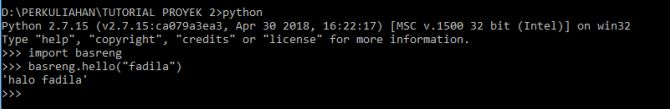
\includegraphics[width=0.70\textwidth]{figures/10/contohsederhana.jpg}}
	    \caption{Fungsi Sederhana}
	    \label{fig:contohsederhana}
  \end{figure}

ini adalah contoh untuk pengeksekusian file python yang berupa gunsi yang telah dibuat. Berikut langkah-langkahnya :
    \begin{itemize}
        \item Petama-tama masukkan kedalam directory tempat anda menyimpan file yang telah anda buat.
        \item kemudian pada directory tersebut ketik python
        \item Setelah masuk kedalam python silahkan masukkan file python basreng
    \end{itemize}

  \item Contoh kasus 2 : Kode pembawa sinyal gelombang otak (NeuroSky Mindwave EEG). Kodenya seperti contoh \ref{lst:coba}, silahkan tutorialnya diikuti terlebih dahulu.
\lstinputlisting[caption=Contoh kode untuk membaca sinyal gelombang otak,label={lst:coba}]{src/10/coba.py}
\end{enumerate}

